%{\color{red} 
%- how does OS manage memory\\
%- page tablesi and hugepages (take it from Jeff's paper)\\
%- GPU page tables\\
%- how does migration happen\\
%- GPU programming and CUDA\\
%}
%
Systems using heterogeneous CPU and GPU computing resources have been widely
used for several years.
%Until recently, the GPU has been managed as a separate
%accelerator, requiring explicit memory management by the programmer to transfer
%data to and from the GPU's address space and (typically) the GPU's
%locally-attached memory.  To increase programmer productivity and broaden the
%classes of workloads that the GPU can execute, recent systems have introduced
%automatic memory management enabling the CPU and GPU to access a unified address
%space and transparently migrate data at a page-level granularity~\cite{UVM}.
%The next step in this evolution is making the GPU a cache-coherent peer to the
%CPU in the memory system, which is the stated goal of a number of commercial
%vendors~\cite{HSA}.
High performance GPUs have developed into stand-alone PCIe-attached
accelerators requiring explicit memory management by the programmer to control
data transfers into the GPU's high-bandwidth locally attached memory. As GPUs
have evolved, the onus of explicit memory management has been addressed by
providing a unified shared memory address space between the GPU and
CPU~\cite{UVM,HSA}.  Whereas a single unified virtual address space improves
programmer productivity, discrete GPU and CPU systems still have separate
locally attached physical memories, optimized for bandwidth and latency
respectively. 


\begin{figure}[t]
    \centering
    \subfloat[Bandwidth sensitivity] {
        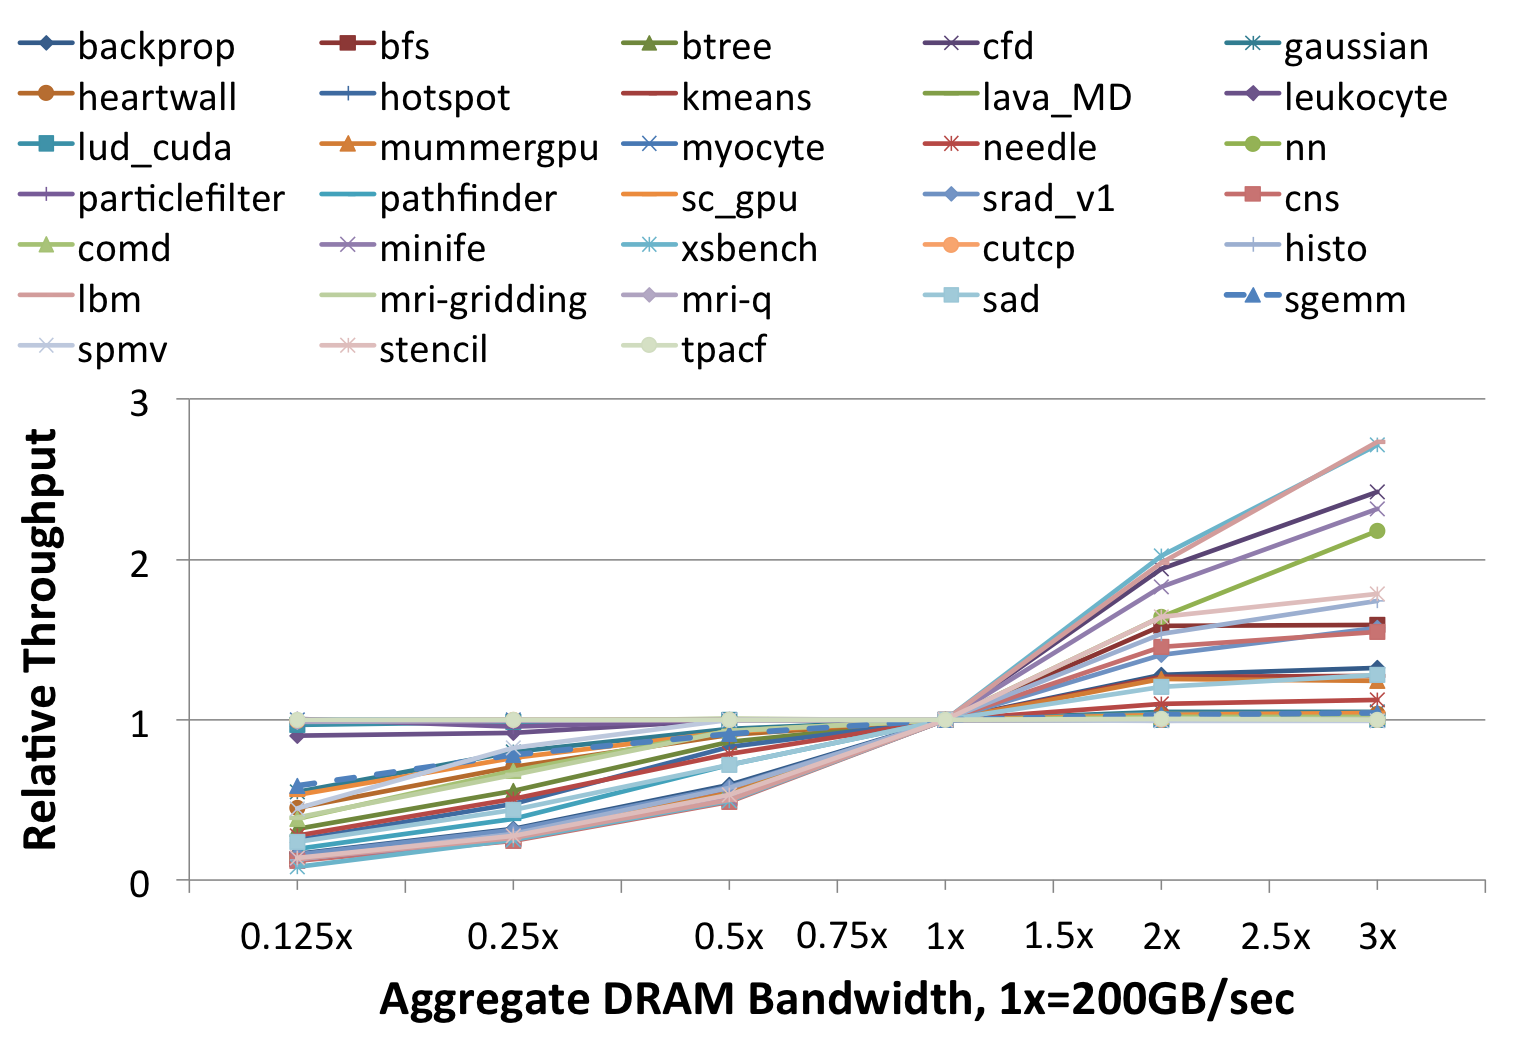
\includegraphics[width=0.8\columnwidth]{asplos2015/figures/bandwidth-1.png}
        \label{fig:bandwidth}
    }
    \\
    \subfloat[Latency sensitivity] {
        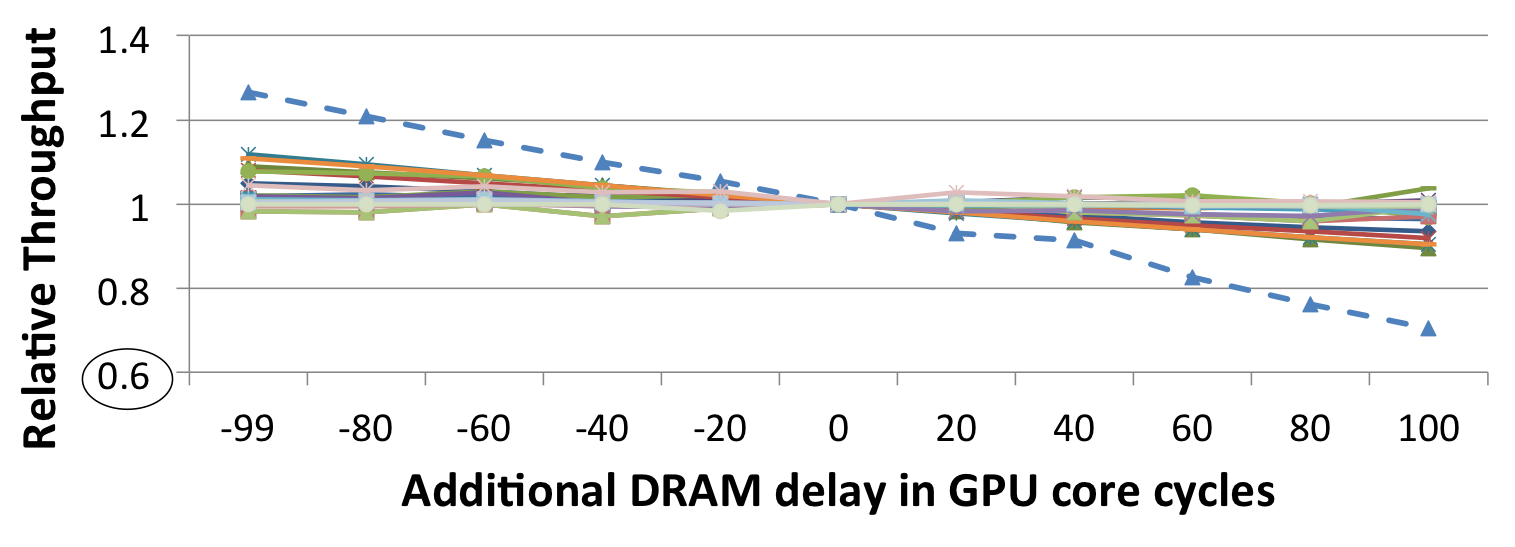
\includegraphics[width=0.8\columnwidth]{asplos2015/figures/latency-1.png}
        \label{fig:latency}
    }
    \caption{GPU performance sensitivity to bandwidth and latency changes.}
    \label{fig:bwlatencysensitivity}
\end{figure}

\section{Bandwidth Hungry Characteristics of GPUs}
%\subsection{{Heterogeneous CC-NUMA Systems}}
\label{heterogeneous_background}
%While some heterogeneous CPU/GPU systems share a single unified physical
%memory~\cite{AMDAPU}, discrete GPUs are already using specialized DRAM optimized
%to meet their high bandwidth demands.
A by-product of the GPU's many-threaded design is that it is able to maintain a
large number of in-flight memory requests and execution throughput is correlated
to memory bandwidth rather than latency, as compared to CPU designs.  As a
result, GPUs have chosen to integrate high bandwidth off-package memory like
GDDR rather than accessing the CPU's DDR directly or integrating DDR locally on
the GPU board. 

To highlight the sensitivity of GPU performance to memory characteristics,
Figures~\ref{fig:bandwidth} and~\ref{fig:latency} show the performance variation
as memory bandwidth and latency vary for a variety of GPU compute benchmarks
from the Rodinia~\cite{Che2009} and {\color{black}Parboil~\cite{Parboil} suites,
as well as a number of recent HPC~\cite{comd,cns,minife,xsbench} workloads. Most
of these GPU workloads are sensitive to changes in bandwidth, while showing much
more modest sensitivity to varying the latency; only {\tt sgemm} stands out as
highly latency sensitive among these 33 workloads. Some application kernels are
neither bandwidth nor latency sensitive and do not see significant performance
variation as modifications are made to the memory subsystem.} While GPU-equipped
systems generally require bandwidth-optimized memories to achieve peak
performance, these memory technologies have significant cost, capacity, and/or
energy disadvantages over alternative DRAM technologies.

The most common Bandwidth-Optimized (BO) memory technology today is
GDDR5~\cite{GDDR5}.  Providing a per-pin data rate of up to 7Gbps, this memory
technology is widely used with discrete GPUs used in HPC, workstation, and
desktop systems.  Due to the high data rates, GDDR5 systems require significant
energy per access and are unable to support high-capacity multi-rank systems.
In contrast, the roadmap for the next several years of cost/capacity-optimized
(CO) DRAM (DDR4 and LPDDR4) provides a per-pin data rate that reaches only 3.2
Gbps.  However, these CO DRAM technologies provide similar latency at a fraction
of the cost and lower energy per access compared to the BO GDDR5 memories.
Looking forward, systems requiring more bandwidth and/or reduced energy per
access are moving to  die-stacked DRAM technologies~\cite{HBM,WIDEIO2}.  These
bandwidth-optimized stacked memories are significantly more energy-efficient
than off-package memory technologies like GDDR5, DDR4, and LPDDR4.
Unfortunately, the number of DRAM die that can be economically stacked in a
single package is limited, necessitating systems to also provide a pool of
off-package capacity-optimized DRAM.

This disaggregation of memory into on-package and off-package pools is one
factor motivating the need to revisit page placement within the context of GPU
performance.  Future GPU/CPU systems are likely to take this disaggregation
further and move capacity-optimized memory not just off the GPU package, but
across a high speed interconnect where it is physically attached to the CPU
rather than the GPU, or possibly further~\cite{limchang09}.  In a CC-NUMA
system, the physical location of this capacity-optimized memory only changes the
latency and bandwidth properties of this memory pool -- it is functionally
equivalent regardless of being CPU or GPU locally attached.  A robust page
placement policy for GPUs will abstract the on-package, off-package, and remote
memory properties into performance and power characteristics based on which it
can make optimized decisions.

\section{Current OS NUMA Page Placement}
\label{linux_background}
%\vspace{-0.05in}
In modern symmetric multiprocessor (SMP) systems, each socket typically consists
of several {\color{black}cores} within a chip multi-processor (CMP) that share
last-level caches and on-chip memory controllers~\cite{INTELXEON}. The number of
memory channels connected to a processor socket is often limited by the
available pin count.  To increase the available memory bandwidth and capacity in
a system, individual sockets can be connected via a cache coherent interconnect
fabric such as Intel's Quick Path~\cite{INTELQPI}, AMD's
HyperTransport~\cite{AMDHT}, or NVIDIA's NVLink~\cite{NVLINK}.  A single socket,
the processors within it, and the physically attached memory comprise what an
operating system sees as a local NUMA zone.  Each socket is a separate NUMA
zone. While a processor within any given zone can access the DRAM within any
other zone, there is additional latency to service this memory request compared
to a locally serviced memory request because the request must be routed first to
its own memory controller, across the socket interconnect, and through the
remote memory controller.

Operating systems such as Linux have recognized that, unless necessary, it is
typically better for applications to service memory requests from their own NUMA
zone to minimize memory latency.  To get the best performance out of these NUMA
systems, Linux learns system topology information from the Advanced
Configuration and Power Interface (ACPI) System Resource Affinity Table (SRAT)
and memory latency information from the ACPI System Locality Information Table
(SLIT)\@. After discovering this information, Linux provides two basic page
placement policies that can be specified by applications to indicate where they
prefer their physical memory pages to be placed when using standard {\tt malloc}
and {\tt mmap} calls to allocate memory.

\emph{LOCAL:} The default policy inherited by user processes is \emph{LOCAL} in
which physical page allocations will be from memory within the local NUMA zone
of the executing process, unless otherwise specified or due to capacity
limitations.  This typically results in allocations from memory physically
attached to the CPU on which the process is running, thus minimizing memory
access latency.

\emph{INTERLEAVE:} The second available allocation policy, which processes must
specifically inform the OS they would like to use, is \emph{INTERLEAVE}\@. This
policy allocates pages round-robin across all (or a subset) of the NUMA zones
within the SMP system to balance bandwidth across the memory pools.  The
downside of this policy is that the additional bandwidth comes at the expense of
increased memory latency. Today, the OS has no knowledge about the relative
bandwidth of memories in these different NUMA zones because SMP systems have
traditionally had bandwidth-symmetric memory systems.

In addition to these OS placement policies, Linux provides a library interface
called \textit{libNUMA} for applications to request memory allocations from
specific NUMA zones.  This facility provides low-level control over memory
placement but requires careful programming because applications running on
different systems will often have different NUMA-zone layouts.  Additional
difficulties arise because there is no performance feedback mechanism available
to programmers when making memory placement decisions, nor are they aware of
which processor(s) their application will be running on while writing their
application.

With the advent of heterogeneous memory systems, the assumptions that operating
system NUMA zones will be symmetric in bandwidth and power
characteristics break down.  The addition of heterogeneous GPU and CPU computing
resources further stresses the page placement policies since processes may not
necessarily be migrated to help mitigate performance imbalance, as certain
phases of computation are now pinned to the type of processor executing the
program.  As a result, data placement policies combined with
bandwidth-asymmetric memories can have significant impact on GPU, and possibly
CPU, performance.

\begin{figure}[t]
    \centering
    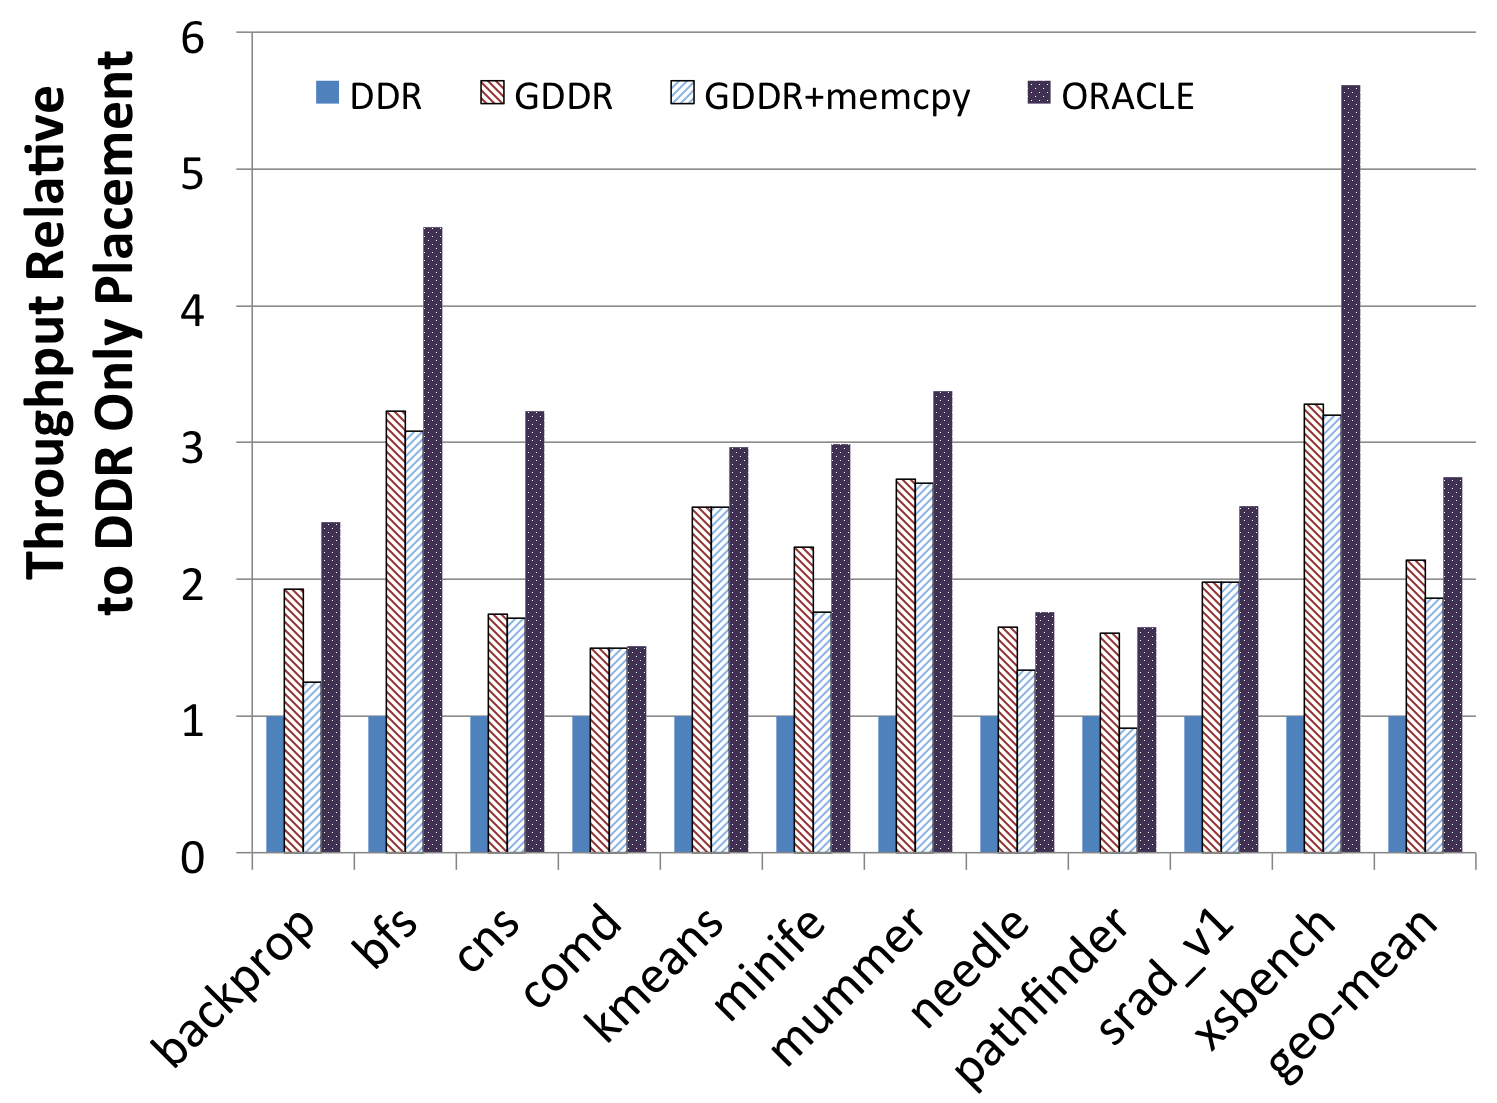
\includegraphics[width=0.7\columnwidth]{hpca2015/figures/motivation.png}
    \caption{GPU performance sensitivity to memory subsystem performance where GDDR provides 
    200GB/s, DDR provides 80GB/s, and {\tt memcpy} bandwidth is 80GB/s.}
    \label{fig:motivation-hpca2015}
\end{figure}

%A by-product of the GPU's many-threaded design is that it is able to maintain a
%large number of in-flight memory requests and execution throughput is correlated
%to memory bandwidth rather than latency, as compared to CPU designs.  As a
%result, GPUs have chosen to integrate high bandwidth off-package memory like
%GDDR rather than accessing the CPU's DDR directly or integrating DDR locally on
%the GPU board.  This choice is motivated by our observation that the performance
%of some GPU compute workloads would degrade by as much as 66\% if the
%traditional GDDR memory on a GPU were replaced with standard DDR memory, as seen
%in Figure~\ref{fig:motivation}.

\section{Memory Copy Overhead in GPUs}
In current CPU/GPU designs, GPU and CPU memory systems are private and require
explicit copying to the GPU before the application can execute.
Figure~\ref{fig:motivation-hpca2015} shows the effect of this copy overhead on
application performance by comparing GDDR to GDDR+{\tt memcpy} performance which
includes the cost of the programmer manually copying data from the DDR to the
GDDR before launching the GPU kernels.  While this copy overhead varies from
application to application, it can be a non-trivial performance overhead for
short-running GPU applications and can even negate the effectiveness of using
the high bandwidth GDDR on-board the GPU in a limited number of cases.

While it is technically possible for the GPU to access CPU memory directly over
PCIe today, the long latency (microseconds) of the access makes this a rarely
used memory operation.  Programming system advancements enabling a uniform
global address space, like those introduced in CUDA 6.0~\cite{cuda}, relax the
requirement forcing programmers to allocate and explicitly copy memory to the
GPU up-front, but do nothing to improve the overhead of this data transfer.
Further, by copying pages from the CPU to the GPU piece-meal on demand, these
new runtimes often introduce additional overhead compared to performing a highly
optimized bulk transfer of all the data that the GPU will need during execution.
The next step in the evolution of GPUs, given the unified addressing, is to
optimize the performance of this new programming model. 

\section {Cache Coherent GPUs Enhancing System Programmability}
The key advancement expected to enable performance is the introduction of
CC-NUMA GPU and CPU systems.  Using cache coherence layered upon NVLink, HT, or
QPI, GPUs will likely be able to access CPU memory in hundreds of nanoseconds at
bandwidths up to 128GB/s by bringing cache lines directly into GPU caches.
Figure~\ref{fig:motivation-hpca2015} shows the upper bound (labeled ORACLE) on
performance that could be achieved if both the system DDR memory and GPU GDDR
memory were used concurrently, assuming data had been optimally placed in both
technologies.  In this work, we define oracle placement to be \emph{a priori}
page placement in the GPU memory (thus requiring no migration), of the minimum
number of pages, when sorted from hottest to coldest, such that the GDDR
bandwidth is fully subscribed during application execution.

Because initial CPU/GPU CC-NUMA systems are likely to use a form of IOMMU
address translation services for walking the OS page tables within the GPU,  it
is unlikely that GPUs will be able to directly allocate and map their own
physical memory without a call back to the CPU and operating system.  In this
work, we make a baseline assumption that all physically allocated pages are
initially allocated in the CPU memory and only the operating system or GPU
runtime system executing on the host can initiate page migrations to the GPU\@.
In such a system, two clear performance goals become evident.  The first is to
design a memory policy that balances CC-NUMA access and page migration to simply
achieve the performance of the legacy bulk copy interface without the
programming limitations.  The second, more ambitious, goal is to exceed this
performance and approach the oracular performance by using these memory zones
concurrently, enabling a peak memory bandwidth that is the sum of the two zones.

Achieving either of these goals requires migrating enough data to the GPU to
exploit its high memory bandwidth while avoiding migrating pages that may never
be accessed again.  Every page migration increases the total bandwidth
requirement of the application and over-migration potentially reduces
application performance if sufficient bandwidth headroom in both the DDR and
GDDR is not available.  Thus, the runtime system must be selective about which
pages to migrate.  The runtime system also must be cognizant that performing TLB
invalidations (an integral part of page migration) on a GPU does not just halt a
single processor, but thousands of compute pipelines that may be accessing these
pages through a large shared TLB structure.  This shared TLB structure makes
page migrations between a CPU and GPU potentially much more costly (in terms of
the opportunity cost of lost execution throughput) than in CPU-only systems.

In addition to managing the memory bandwidth overhead of page migration and
execution stalls due to TLB shootdowns, the relative bandwidth utilization of
both the CPU and GPU memory must be taken into account when making page
migration decisions.  When trying to balance memory bandwidth between two
distinct memory zones, it is possible to over- or under-subscribe either memory
zone. Migrating pages too slowly to the GPU memory will leave its local memory
sitting idle, wasting precious bandwidth.  Conversely, migrating pages to the
GPU too aggressively may result in under-utilization of the CPU memory while
paying the maximum cost in terms of migration overheads. A comprehensive CPU-GPU
memory management solution will attempt to balance all of these effects to
maximize memory system and GPU throughput in future mobile, graphics, HPC, and
data-center installations.

\section{Supporting Hardware Cache Coherence in GPUs}
%Heterogeneous CPU--GPU systems have been widely adopted by the high performance
%computing community and are becoming increasingly common in other computing
%paradigms. High performance GPUs have developed into stand-alone PCIe-attached
%accelerators requiring explicit memory management by the programmer to control
%data transfers into the GPU's high-bandwidth locally attached memory. As GPUs
%have evolved, the onus of explicit memory management has been addressed by
%providing a unified shared memory address space between the GPU and
%CPU~\cite{UVM,HSA}.  Whereas a single unified virtual address space improves
%programmer productivity, discrete GPU and CPU systems still have separate
%locally attached physical memories, optimized for bandwidth and latency
%respectively. 

Managing the physical location of data, and guaranteeing that reads access the
most up-to-date copies of data in a unified shared memory can be done through
the use of page level migration and protection. Such mechanisms move data at the
OS page granularity between physical memories~\cite{UVM}.  With the advent of
non-PCIe high bandwidth, low latency CPU--GPU interconnects, the possibility of
performing cache-line, rather than OS-page-granularity, accesses becomes
feasible.  Without OS level page protection mechanisms to support correctness
guarantees, however,  the responsibility of coherence has typically fallen on
hardware cache-coherence implementations.

\begin{table}[t]
\begin{center}
\begin{tabular}{ddd}
 \hline
 \multicolumn{1}{l}{Workload} &   \multicolumn{1}{c}{L1 Hit Rate (\%)}  &  \multicolumn{1}{c}{L2 Hit Rate (\%)}  \\
 \hline
 \hline
 \multicolumn{1}{l}{backprop}  &   62.4  &   70.0\\
 \hline
 \multicolumn{1}{l}{bfs}  &   19.6  &   58.6  \\
 \hline
 \multicolumn{1}{l}{btree}  &   81.8  &   61.8  \\
 \hline
 \multicolumn{1}{l}{cns}  &   47.0  &   55.2  \\
 \hline
 \multicolumn{1}{l}{comd}  &   62.5  &   97.1  \\
 \hline
 \multicolumn{1}{l}{kmeans}  &   5.6  &   29.5  \\
 \hline
 \multicolumn{1}{l}{minife}  &   46.7  &   20.4  \\
 \hline
 \multicolumn{1}{l}{mummer}  &   60.0  &   30.0  \\
 \hline
 \multicolumn{1}{l}{needle}  &   7.0  &   55.7  \\
 \hline
 \multicolumn{1}{l}{pathfinder}  &   42.4  &   23.0  \\
 \hline
 \multicolumn{1}{l}{srad\_v1}  &   46.9  &   25.9  \\
 \hline
 \multicolumn{1}{l}{xsbench}  &   30.7  &   63.0  \\
 \hline
 \hline
 \multicolumn{1}{l}{Arith Mean}  &   44.4  &   51.6  \\
\hline
\end{tabular}
\caption{GPU L1 and L2 cache hit rates (average).}
\label{tab:gpuhitrate}
\end{center}
\vspace{-.25in}
\end{table}

\begin{figure*}[t]
    \centering
    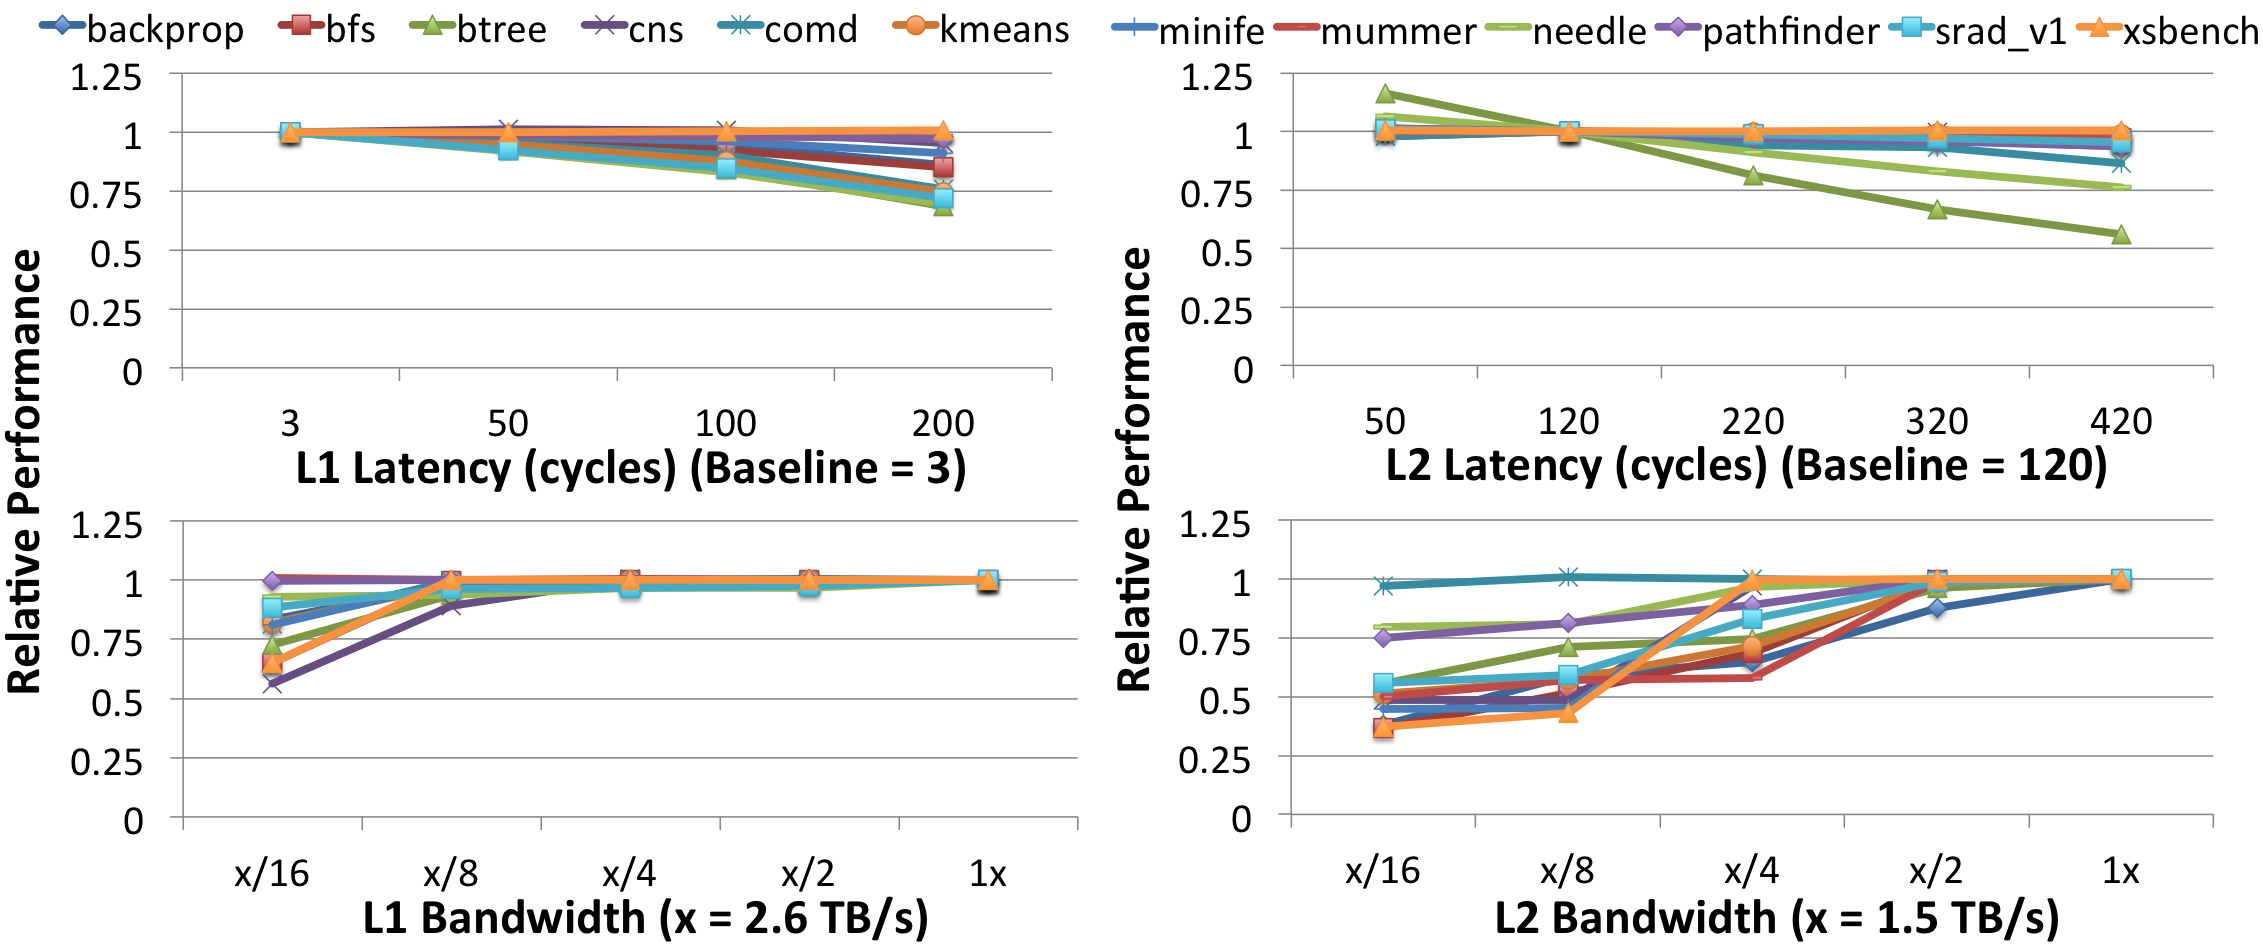
\includegraphics[width=\textwidth]{hpca2016/figures/cache_bw_latency.png}
    \caption{GPU performance sensitivity to L1 and L2 latency and bandwidth
changes.}
    \label{fig:cache_bw_latency}
    \vspace{-.1in}
\end{figure*}

As programming models supporting transparent CPU-GPU sharing become more
prevalent and sharing becomes more fine-grain and frequent, the performance gap
between page-level coherence and fine-grained hardware cache-coherent access
will grow~\cite{Agarwal2015,Agarwal2015b,Lim2012}.  On-chip caches, and thus HW
cache coherence, are widely used in CPUs because they provide substantial memory
bandwidth and latency improvements~\cite{Martin2012}.  Building scalable,
high-performance cache coherence requires a holistic system that strikes a
balance between directory storage overhead, cache probe bandwidth, and
application
characteristics~\cite{Power2013,Pugsley2010,Cantin2005,johnson2011,Hong2012,Sanchez2012,Kelm2010}.
Although relaxed or scoped consistency models allow coherence operations to be
re-ordered or deferred, hiding latency, they do not obviate the need for HW
cache coherence. However, supporting a CPU-like HW coherence model in large
GPUs, where many applications do not require coherence, is a tax on GPU
designers.  Similarly, requiring CPUs to relax or change their HW coherence
implementations or implement instructions enabling software management of the
cache hierarchy adds significant system complexity.

Prior work has shown that due to their many threaded design, GPUs are
insensitive to off-package memory latency but very sensitive to off-chip memory
bandwidth~\cite{Agarwal2015,Agarwal2015b}. Table~\ref{tab:gpuhitrate} shows the
L1 and L2 cache hit rates across a variety of workloads from the Rodinia and
United States Department of Energy application suites~\cite{Che2009,villa2014}.
These low hit rates cause GPUs to also be fairly insensitive to small changes in
L1 and L2 cache latency and bandwidth, as shown in
Figure~\ref{fig:cache_bw_latency}.  This lack of sensitivity raises the question
whether GPUs need to uniformly employ on-chip caching of all off-chip memory in
order to achieve good performance.  If GPUs do not need or can selectively
employ on-chip caching, then CPU--GPU systems can be built that present a
unified coherent shared memory address space to the CPU, while not requiring a
HW cache-coherence implementation within the GPU. 

Avoiding hardware cache coherence benefits GPUs by decoupling them from the
coherence protocol implemented within the CPU complex, enables simplified GPU
designs, and improves compatibility across future systems. It also reduces the
scaling load on the existing CPU coherence and directory structures by
eliminating the potential addition of hundreds of additional caches, all of
which may be sharing data. Selective caching does not come without a cost
however. Some portions of the global memory space will become un-cacheable
within the GPU\@ and bypassing on-chip caches can place additional load on
limited off-chip memory resources.  In the following sections, we show that by
leveraging memory request coalescing, small CPU-side caches, improved
interconnect efficiency, and promiscuous read-only caching, selective caching
GPUs can perform nearly as well as HW cache-coherent CPU--GPU\@ systems.
